\documentclass{report}
\usepackage{comment}
\usepackage{graphicx}
\usepackage{pbox}
\usepackage[section]{placeins}
\usepackage{float}
\usepackage{tablefootnote}
\usepackage{svg}
% \usepackage{flafter} 
\usepackage[colorlinks, linkcolor = black, citecolor = black, filecolor = black, urlcolor = blue]{hyperref} 


\title{
  \Huge - Uncoronainfectify -
  \\ \small (working title)
}

\setcounter{secnumdepth}{5}
\setcounter{tocdepth}{4}


\author{
  $$Group 9$$
}
\begin{document}
  \maketitle
  \tableofcontents
  \newpage
  
  \chapter{Introduction}

  \section{Purpose}
  
The purpose of this document.

  \section{Scope}
  Scopedi Scope.

 \newpage
  \section{Definitions, acronyms and abbreviations}
  \begin{table}[!h]
    \caption{Data Dictionary}
        \label{tab:Table1}
        \begin{tabular}{l|p{2cm}|p{10cm}}
            \textbf{Number} & \textbf{Term} & \textbf{Definition}\\
            \hline 1 & Functional requirement & What the system should do \\
            \hline 2 & Non-functional requirement & How the system should do something (e.g. fast) \\
            \hline 3 & Shall & Requirements marked with “shall” must be implemented and verified \\
            \hline 4 & Will & Requirements marked with “will” must be implemented and cannot/will not be verified \\
            \hline 5 & Should & Requirements marked with “should” must be implemented and cannot/will not be verified \\
        \end{tabular}
\end{table}
  
  \section{References}
  \href{https://github.com/FontysVenlo/prj4-2020-app-ios-2020-group09/}{github}  \\
\href{https://en.wikipedia.org/wiki/Road_traffic_control/}{Wikipedia.org Road traffic control}  \\
\href{/}{.}  \\   

  \section{Overview}
  
\begin{itemize}
    \item item
    \item  item
    
\end{itemize}
Stuff

  \newpage
  
\chapter{Overall description}
    
  \section{Product perspective}
  \begin{figure}[H]
    \centering
    \caption{Diagram}
    % \includegraphics[height=300px]{block_diagram.pdf}
\end{figure}

  % \section{Interfaces}
  \subsection{User interfaces}
    Not applicable to our program

\subsection{Hardware interfaces}
    \begin{itemize}
        \item item
    \end{itemize}
    Stuff

\subsection{Software interfaces}
    \begin{itemize}
        \item item
    \end{itemize}
    Stuff

\subsection{Communication interfaces}
    Stuff

\subsection{System interfaces}
    No System interfaces

\subsection{Memory Constraints}
    No memory Constraints

\subsection{Site adaption requirements}
    \begin{itemize}
        \item Stuff
    \end{itemize}

  \newpage
  \section{Product functions}
  \begin{figure}[H]
    \centering
        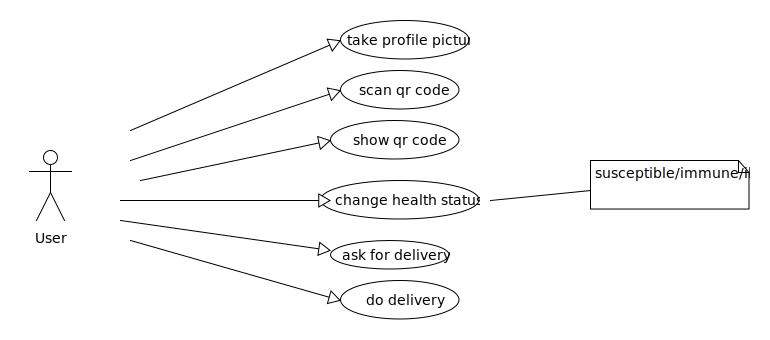
\includegraphics[height=350px]{resources/use_case_diagram.pdf}    
    \caption{Use Case Diagram}
    \label{}
\end{figure}
% Standart layout of a use case description



	


\begin{comment}
\vspace{5mm}

\begin{table}[H]
    \begin{tabular}{ |p{2cm}||p{11cm}| }
        \hline
        \multicolumn{2}{|c|}{$$Login$$} \\ \hline
        \textbf{ID} & \textbf{UC01} \\ \hline
        Actor & test \\ \hline
        Precondition & test \\ \hline
        Scenario &
        \begin{enumerate}
            \item actor
            \item system
        \end{enumerate}
        \\ \hline 
        Exceptions & test \\ \hline
        Extensions & test \\ \hline
        Result & test \\ \hline
    \end{tabular}
    \caption{Use Case Description: "Description"}
\end{table}



\end{comment}
\newpage
\subsection{Use Case Descriptions}

\begin{center}
    \vspace{5mm}
    \begin{table}[H]
        \begin{tabular}{ |p{2cm}||p{11cm}| }
            \hline
            \multicolumn{2}{|c|}{$$Use Case$$ - Create an account} \\ \hline
            \textbf{ID} & \textbf{UC01} \\ \hline
            Actor & User \\ \hline
            Precondition & - \\ \hline
            Scenario &
            \begin{enumerate}
                \item ACTOR initiates the application
                \item SYSTEM directs to the launch space
                \item ACTOR navigates to the create an account section
                \item SYSTEM displays create an account section
                \item ACTOR fills in desired credentials and asks SYSTEM to process the form
                \item SYSTEM verifies the filled in credentials and outputs a validation message
            \end{enumerate}
            \\ \hline 
            Exceptions & 6. Filled in credentials are incorrect \\ \hline
            Extensions & None \\ \hline
            Result & ACTOR is logged into the application using their credentials \\ \hline
        \end{tabular}
        \caption{Use Case Description: "Create an account"}
    \end{table}

    \vspace{5mm}
    \begin{table}[H]
        \begin{tabular}{ |p{2cm}||p{11cm}| }
            \hline
            \multicolumn{2}{|c|}{$$Use Case$$ - Log in} \\ \hline
            \textbf{ID} & \textbf{UC02} \\ \hline
            Actor & User \\ \hline
            Precondition & Actor has an account \\ \hline
            Scenario &
            \begin{enumerate}
                \item ACTOR initiates the application
                \item SYSTEM directs to the launch space
                \item ACTOR inputs credentials
                \item SYSTEM verifies credentials
            \end{enumerate}
            \\ \hline 
            Exceptions &  4. SYSTEM displays message that credentials are incorrect\\ \hline
            Extensions & None \\ \hline
            Result & User is logged in \\ \hline
        \end{tabular}
        \caption{Use Case Description: "Log in"}
    \end{table}
    
    \vspace{5mm}
    \begin{table}[H]
        \begin{tabular}{ |p{2cm}||p{11cm}| }
            \hline
            \multicolumn{2}{|c|}{$$Use Case$$ - Log out} \\ \hline
            \textbf{ID} & \textbf{UC03} \\ \hline
            Actor & User \\ \hline
            Precondition & Actor is logged in \\ \hline
            Scenario &
            \begin{enumerate}
                \item ACTOR initiates the application
                \item SYSTEM directs to the launch space
                \item ACTOR navigates to log out section
                \item SYSTEM displays option to log out
                \item ACTOR chooses to log out
                \item SYSTEM logs ACTOR out
            \end{enumerate}
            \\ \hline 
            Exceptions & None \\ \hline
            Extensions & None \\ \hline
            Result & User is logged out \\ \hline
        \end{tabular}
        \caption{Use Case Description: "Log out"}
    \end{table}
    
    \vspace{5mm}
    \begin{table}[H]
        \begin{tabular}{ |p{2cm}||p{11cm}| }
            \hline
            \multicolumn{2}{|c|}{$$Use Case$$ - Show QR code} \\ \hline
            \textbf{ID} & \textbf{UC04} \\ \hline
            Actor & User \\ \hline
            Precondition & ACTOR is logged in\\ \hline
            Scenario &
            \begin{enumerate}
                \item ACTOR initiates the application
                \item SYSTEM directs to the launch space
                \item ACTOR navigates to the Show QR code section
                \item SYSTEM displays QR code
            \end{enumerate}
            \\ \hline 
            Exceptions & None \\ \hline
            Extensions & None \\ \hline
            Result & ACTOR is able to see their own QR code \\ \hline
        \end{tabular}
        \caption{Use Case Description: "Show QR code"}
    \end{table}
    
    \vspace{5mm}
    \begin{table}[H]
        \begin{tabular}{ |p{2cm}||p{11cm}| }
            \hline
            \multicolumn{2}{|c|}{$$Use Case$$ - Scan QR code} \\ \hline
            \textbf{ID} & \textbf{UC05} \\ \hline
            Actor & User \\ \hline
            Precondition & ACTOR is logged in \\ \hline
            Scenario &
            \begin{enumerate}
                \item \underline{Show QR code}
                \item ACTOR navigates to scan QR code section
                \item SYSTEM opens camera
                \item ACTOR scans the QR code with use of the camera
                \item SYSTEM outputs a validation message
            \end{enumerate}
            \\ \hline 
            Exceptions & None \\ \hline
            Extensions & None \\ \hline
            Result & QR code has been scanned \\ \hline
        \end{tabular}
        \caption{Use Case Description: "Scan QR code"}
    \end{table}
    
    \vspace{5mm}
    \begin{table}[H]
        \begin{tabular}{ |p{2cm}||p{11cm}| }
            \hline
            \multicolumn{2}{|c|}{$$Use Case$$ - Change health status} \\ \hline
            \textbf{ID} & \textbf{UC06} \\ \hline
            Actor & User \\ \hline
            Precondition & ACTOR is logged in \\ \hline
            Scenario &
            \begin{enumerate}
                \item ACTOR initiates the application
                \item SYSTEM directs to the launch space
                \item ACTOR navigates to Change health status section
                \item SYSTEM displays health status options
                \item ACTOR chooses a health status option
                \item SYSTEM saves updated health status
                
            \end{enumerate}
            \\ \hline 
            Exceptions & None \\ \hline
            Extensions & 6. SYSTEM sends notifications to other users (if health status was changed to sick) \\ \hline
            Result & The health status of the user is updated (other users are notified) \\ \hline
        \end{tabular}
        \caption{Use Case Description: "Change health status"}
    \end{table}
    
    \vspace{5mm}
    \begin{table}[H]
        \begin{tabular}{ |p{2cm}||p{11cm}| }
            \hline
            \multicolumn{2}{|c|}{$$Use Case$$ - Take profile picture} \\ \hline
            \textbf{ID} & \textbf{UC07} \\ \hline
            Actor & User \\ \hline
            Precondition & ACTOR is logged in \\ \hline
            Scenario &
            \begin{enumerate}
                \item ACTOR initiates the application
                \item SYSTEM directs to the launch space
                \item ACTOR navigates to account settings section
                \item SYSTEM displays option to take a profile picture
                \item ACTOR takes a profile picture
                \item SYSTEM saves profile picture
            \end{enumerate}
            \\ \hline 
            Exceptions & None \\ \hline
            Extensions & None \\ \hline
            Result & User has a new profile picture \\ \hline
        \end{tabular}
        \caption{Use Case Description: "Take profile picture"}
    \end{table}
    
    \vspace{5mm}
    \begin{table}[H]
        \begin{tabular}{ |p{2cm}||p{11cm}| }
            \hline
            \multicolumn{2}{|c|}{$$Use Case$$ - Request delivery} \\ \hline
            \textbf{ID} & \textbf{UC08} \\ \hline
            Actor & User \\ \hline
            Precondition & ACTOR is logged in \\ \hline
            Scenario &
            \begin{enumerate}
                \item ACTOR initiates the application
                \item SYSTEM directs to the launch space
                \item ACTOR navigates to the request delivery section
                \item SYSTEM displays the request delivery section
                \item ACTOR fills in information about the desired delivery and processes the result
                \item SYSTEM verifies the filled in information and outputs a validation message
            \end{enumerate}
            \\ \hline 
            Exceptions & 6. Filled in information is incorrect \\ \hline
            Extensions & None \\ \hline
            Result & Delivery request is successfully posted \\ \hline
        \end{tabular}
        \caption{Use Case Description: "Request delivery"}
    \end{table}
    
    \vspace{5mm}
    \begin{table}[H]
        \begin{tabular}{ |p{2cm}||p{11cm}| }
            \hline
            \multicolumn{2}{|c|}{$$Use Case$$ - Execute delivery} \\ \hline
            \textbf{ID} & \textbf{UC09} \\ \hline
            Actor & User \\ \hline
            Precondition & ACTOR is logged in and there must be at least one available request \\ \hline
            Scenario &
            \begin{enumerate}
                \item ACTOR initiates the application
                \item SYSTEM directs to the launch space
                \item ACTOR navigates to the execute delivery section
                \item SYSTEM displays the open delivery requests
                \item ACTOR selects the desired delivery to execute
                \item SYSTEM outputs a validation message
            \end{enumerate}
            \\ \hline 
            Exceptions & None \\ \hline
            Extensions & None \\ \hline
            Result & Delivery request is executed \\ \hline
        \end{tabular}
        \caption{Use Case Description: "Execute delivery"}
    \end{table}

    \vspace{5mm}
    \begin{table}[H]
        \begin{tabular}{ |p{2cm}||p{11cm}| }
            \hline
            \multicolumn{2}{|c|}{$$Use Case$$ - Lookup Meeting} \\ \hline
            \textbf{ID} & \textbf{UC10} \\ \hline
            Actor & User \\ \hline
            Precondition & ACTOR is logged in and had at least one previous meeting \\ \hline
            Scenario &
            \begin{enumerate}
                \item ACTOR initiates the application
                \item SYSTEM directs to the launch space
                \item ACTOR navigates to the lookup meetings section
                \item SYSTEM displays the lookup meeting section
                \item ACTOR selects a meeting he wants to lookup
                \item SYSTEM shows the meetings date and location on a map
            \end{enumerate}
            \\ \hline 
            Exceptions & None \\ \hline
            Extensions & None \\ \hline
            Result & A Previous meeting is displayed \\ \hline
        \end{tabular}
        \caption{Use Case Description: "Lookup Meeting"}
    \end{table}
    
    \end{center}


  \newpage
  \section{User characteristics} % Doc vs Normal Guy
  % \input{overall_description/usercharacteristics.tex}
  
  \newpage
  \section{Constraints}
  \begin{itemize}
  \item item
\end{itemize}


  
  \newpage
  \section{Apportioning of requirements}
  \begin{comment}
\vspace{5mm}
\begin{table}[H]
	\begin{tabular}{ |p{2cm}||p{9cm}| }
		\hline
        ID & \textbf{FREQ005}\\ \hline
        UC & \textbf{UC01} \\ \hline
		Category & functional \\ \hline
		Description &
		
		\\ \hline
		Rationale &  \\ \hline
	\end{tabular}
	\caption{Functional Requirement: ""}
\end{table}
\end{comment}

\vspace{5mm}
\begin{table}[H]
	\begin{tabular}{ |p{2cm}||p{9cm}| }
		\hline
        ID & \textbf{FREQ007}\\ \hline
        UC & \textbf{UC01} \\ \hline
		Category & functional \\ \hline
		Description &
        The user shall be able to view a heatmap of corona infections.
		\\ \hline
		Rationale & Duuuu Duuuu Duuu Duuuu \\ \hline
	\end{tabular}
	\caption{Functional Requirement: "Heatmap"}
\end{table}

In the following Requirements: 
\\ Person A = the one that is in quarantine.
\\ Person B = the shopping queen. 

\vspace{5mm}
\begin{table}[H]
	\begin{tabular}{ |p{2cm}||p{9cm}| }
		\hline
        ID & \textbf{FREQ007}\\ \hline
        UC & \textbf{UC08} \\ \hline
		Category & functional \\ \hline
		Description &
        Person A in quarantine/ in a risk group shall be able to ask a 
        possible person B to do shopping for it.
		\\ \hline
		Rationale & To keep social distance. \\ \hline
	\end{tabular}
	\caption{Functional Requirement: "Delivery"}
\end{table}

\vspace{5mm}
\begin{table}[H]
	\begin{tabular}{ |p{2cm}||p{9cm}| }
		\hline
        ID & \textbf{FREQ008}\\ \hline
        UC & \textbf{UC09} \\ \hline
		Category & functional \\ \hline
		Description &
		Person B shall only see shopping lists of Person As that are in a 30km radius. 
		\\ \hline
		Rationale & Do not spread infections even more. \\ \hline
	\end{tabular}
	\caption{Functional Requirement: "Localization"}
\end{table}

\vspace{5mm}
\begin{table}[H]
	\begin{tabular}{ |p{2cm}||p{9cm}| }
		\hline
        ID & \textbf{FREQ009}\\ \hline
        UC & \textbf{UC08} \\ \hline
		Category & functional \\ \hline
		Description &
		Person A shall be able to specify a shopping list. (Keep it simple)
		\\ \hline
		Rationale & So B knows what to get. \\ \hline
	\end{tabular}
	\caption{Functional Requirement: "Shopping List"}
\end{table}

\vspace{5mm}
\begin{table}[H]
	\begin{tabular}{ |p{2cm}||p{9cm}| }
		\hline
        ID & \textbf{FREQ010}\\ \hline
        UC & \textbf{UC09} \\ \hline
		Category & functional \\ \hline
		Description &
        Person B shall be able to confirm the request for a shopping list. 
        This means he is accepting to buy everything from the list.
		\\ \hline
		Rationale & So it is removed from the shopping list pool. \\ \hline
	\end{tabular}
	\caption{Functional Requirement: "Confirm shopping"}
\end{table}

\vspace{5mm}
\begin{table}[H]
	\begin{tabular}{ |p{2cm}||p{9cm}| }
		\hline
        ID & \textbf{FREQ012}\\ \hline
        UC & \textbf{UC08} \\ \hline
		Category & functional \\ \hline
		Description &
		Person A shall be able to confirm that Person B has done the shopping.
		\\ \hline
		Rationale & To change the state to delivered. \\ \hline
	\end{tabular}
	\caption{Functional Requirement: "Shopping done"}
\end{table}

  \newpage
  \section{Assumptions \& Dependencies}
  This Section of the IEEE 830-1998 standard is not applicable for this document.
  \newpage
  
\chapter{Specific Requirements}



  \section{External interface requirements}
  This Section of the IEEE 830-1998 standard is not applicable for this document. 
\vspace{5mm}

  \section{Functional Requirements}
  
  \begin{comment}

\vspace{5mm}
\begin{table}[H]
	\begin{tabular}{ |p{2cm}||p{9cm}| }
		\hline
        ID & \textbf{FREQ005}\\ \hline
        UC & \textbf{UC01} \\ \hline
		Category & functional \\ \hline
		Description &
		
		\\ \hline
		Rationale &  \\ \hline
	\end{tabular}
	\caption{Functional Requirement: ""}
\end{table}
\end{comment}

% UC 01

\vspace{5mm}
\begin{table}[H]
	\begin{tabular}{ |p{2cm}||p{9cm}| }
		\hline
        ID & \textbf{FREQ000}\\ \hline
        UC & \textbf{UC07} \\ \hline
		Category & functional \\ \hline
		Description &
		A user shall be able to add a profile picture via the app.
		\\ \hline
		Rationale & To make it use the camera. \\ \hline
	\end{tabular}
	\caption{Functional Requirement: "Facetime"}
\end{table}

\begin{flushleft}
    \vspace{5mm}
\begin{table}[H]
    \begin{tabular}{ |p{2cm}||p{9cm}| }
        \hline
        ID & \textbf{FREQ001\tablefootnote{Functional Requirement}}\\ \hline
        UC\tablefootnote{Associated Usecase} & \textbf{UC01, UC02} \\ \hline
        Category & functional \\ \hline
        Description & 
        The account shall be uniquely identified by the users phonenumber. 
        The number shall be captured by the phone automatically.
        Login shall be automated.
        \\ \hline
        Rationale & For unique identification and to prevent multiple accounts per user. \\ \hline 
    \end{tabular} 
\caption{Functional Requirement: "Login with phone number"}
\end{table}

\vspace{5mm}
\begin{table}[H]
	\begin{tabular}{ |p{2cm}||p{9cm}| }
		\hline
        ID & \textbf{FREQ003}\\ \hline
        UC & \textbf{UC05} \\ \hline
		Category & functional \\ \hline
		Description &
		A user shall be able to scan another users/places QR-code.
		\\ \hline
		Rationale & To keep track of the locations/persons he met. \\ \hline
	\end{tabular}
	\caption{Functional Requirement: "Scan QR-code"}
\end{table}

\vspace{5mm}
\begin{table}[H]
	\begin{tabular}{ |p{2cm}||p{9cm}| }
		\hline
        ID & \textbf{FREQ004}\\ \hline
        UC & \textbf{UC05} \\ \hline
		Category & functional \\ \hline
		Description &
        If A scans B's QR-code, both users shall be linked/marked as in close contact.
        This means the B does not have to scan A's QR-code as well.
		\\ \hline
		Rationale & To minimise contact. \\ \hline
	\end{tabular}
	\caption{Functional Requirement: "Scan just once"}
\end{table}

\vspace{5mm}
\begin{table}[H]
	\begin{tabular}{ |p{2cm}||p{9cm}| }
		\hline
        ID & \textbf{FREQ005}\\ \hline
        UC & \textbf{UC06} \\ \hline
		Category & functional \\ \hline
		Description &
        A user shall be able to switch its' health status. 
        Possible states: susceptible, ill, immune.
		\\ \hline
		Rationale & To be able to notify users that scanned each others barcodes. \\ \hline
	\end{tabular}
	\caption{Functional Requirement: "Switch health status"}
\end{table}

\vspace{5mm}
\begin{table}[H]
	\begin{tabular}{ |p{2cm}||p{9cm}| }
		\hline
        ID & \textbf{FREQ006}\\ \hline
        UC & \textbf{UC04} \\ \hline
		Category & functional \\ \hline
		Description &
		A user shall be able to display its QR code. 
		\\ \hline
		Rationale & To make it scannable. \\ \hline
	\end{tabular}
	\caption{Functional Requirement: "Show QR-code"}
\end{table}

% % GPS related

\vspace{5mm}
\begin{table}[H]
	\begin{tabular}{ |p{2cm}||p{9cm}| }
		\hline
        ID & \textbf{FREQ007}\\ \hline
        UC & \textbf{SHOW MEETINGS} \\ \hline
		Category & functional \\ \hline
		Description &
		A user shall be able to see all his previous meetings.
		A meeting should be displayed on a map.
		\\ \hline
		Rationale & asdf \\ \hline
	\end{tabular}
	\caption{Functional Requirement: "See previous meetings"}
\end{table}

\vspace{5mm}
\begin{table}[H]
	\begin{tabular}{ |p{2cm}||p{9cm}| }
		\hline
        ID & \textbf{FREQ008}\\ \hline
        UC & \textbf{SHOW MEETINGS} \\ \hline
		Category & functional \\ \hline
		Description &
		The user shall see the Persons name he met with in a previous meeting.
		The name could be taken from the contacts list/phonenumber.
		\\ \hline
		Rationale & To keep track of you meetings. \\ \hline
	\end{tabular}
	\caption{Functional Requirement: "See your doomed friends names"}
\end{table}

% Tracablility Matrix
\begin{table}[H]    
    \begin{tabular}{|p{2.5cm}|p{0.5cm}|p{0.5cm}|p{0.5cm}|p{0.5cm}|p{0.5cm}|p{0.5cm}|p{0.5cm}|p{0.5cm}|} 
        \hline & \textbf{01} & \textbf{02} & \textbf{03} & \textbf{04} & \textbf{05} & \textbf{06} & \textbf{07} & \textbf{08} \\ \hline
        %                  1  2  3  4  5  6  7  8  
        \textbf{FREQ001} & x& x& x& x& x& x& x& x\\ \hline
        \textbf{FREQ002} & x& x&  &  &  &  &  &  \\ \hline
        \textbf{FREQ003} & x& x& x& x& x& x& x& x\\ \hline
        \textbf{FREQ004} & x& x& x& x& x& x& x& x\\ \hline
        \textbf{FREQ005} &  &  & x& x& x& x& x& x\\ \hline
        \textbf{FREQ006} &  &  &  &  & x&  &  & x\\ \hline
        \textbf{FREQ007} &  &  &  &  & x&  &  & x\\ \hline
        \textbf{FREQ008} &  &  &  & x& x&  &  &  \\ \hline
        \textbf{FREQ009} &  &  &  &  & x& x& x& x\\ \hline
        \textbf{FREQ010} &  &  &  &  & x&  &  & x\\ \hline
        \textbf{FREQ011} &  &  &  & x&  &  &  & x\\ \hline
        \textbf{FREQ012} &  &  & x&  & x&  &  & x\\ \hline
        \textbf{FREQ013} &  &  & x&  & x&  &  & x\\ \hline
		\textbf{FREQ014} & x& x&  & x&  &  &  & x\\ \hline
		\textbf{FREQ015} & x& x&  & x&  &  &  & x\\ \hline
        \textbf{FREQ016} &  &  &  &  & x& x&  & x\\ \hline
        \textbf{FREQ017} &  &  &  &  & x&  &  & x\\ \hline
        \textbf{FREQ018} &  &  &  &  &  &  &  &  \\ \hline
        \textbf{FREQ019} &  &  &  &  &  &  &  &  \\ \hline
        \textbf{FREQ020} &  &  &  &  &  &  &  &  \\ \hline
        \textbf{FREQ021} &  &  &  &  & x&  &  & x\\ \hline
        % \textbf{FREQ022} & x& x& x& x& x& x& x& x\\ \hline
        
        % \textbf{foo} &  &  &  &  &  &  &  &  \\ \hline
    \end{tabular}
    \caption{Tracablility Matrix for Functional Requirements}
\end{table}

\end{flushleft}


  \newpage

  \section{Non-Functional requirements}
  \begin{comment}
\vspace{5mm}
    
\begin{tabular}{ |p{2cm}||p{9cm}| }
    \hline
    ID & \textbf{PREQ000}\\ \hline
    Category & performance \\ \hline
    Description & 

    \\ \hline
    Rationale &  \\ \hline 
    Source &  \\ \hline
\end{tabular}  
\end{comment}

\begin{flushleft}

\vspace{5mm}
\begin{table}[H]
    \begin{tabular}{ |p{2cm}||p{9cm}| }
        \hline
        ID & \textbf{UPREQ001}\\ \hline
        Category & Nonfunctional \\ \hline
        Description & 
        Users can only have one account per iOS device.
        \\ \hline
        Rationale & To avoid multiple accounts per user. \\ \hline 
    \end{tabular} 
\caption{Use Case Requirement: "One Account/Person"}
\end{table}

\vspace{5mm}
\begin{table}[H]
    \begin{tabular}{ |p{2cm}||p{9cm}| }
        \hline
        ID & \textbf{UPREQ002}\\ \hline
        Category & Nonfunctional \\ \hline
        Description & 
        Application should be implemented asynchronously.
        \\ \hline
        Rationale & Avoid long loading times/frezes. \\ \hline 
    \end{tabular} 
\caption{Use Case Requirement: "Asynchron"}
\end{table}

\vspace{5mm}
\begin{table}[H]
    \begin{tabular}{ |p{2cm}||p{9cm}| }
        \hline
        ID & \textbf{UPREQ003}\\ \hline
        Category & Nonfunctional \\ \hline
        Description & 
        The UI should be easy to use.
        \\ \hline
        Rationale & elderly people. \\ \hline 
    \end{tabular} 
\caption{Use Case Requirement: "Old People"}
\end{table}

\vspace{5mm}
\begin{table}[H]
    \begin{tabular}{ |p{2cm}||p{9cm}| }
        \hline
        ID & \textbf{UPREQ004}\\ \hline
        Category & Nonfunctional \\ \hline
        Description & 
        The users data should be pseudonymised.
        \\ \hline
        Rationale & GDPR. \\ \hline 
    \end{tabular} 
\caption{Use Case Requirement: "GDPR"}
\end{table}

% Tracablility Matrix
\begin{table}[H]    
    \begin{tabular}{|p{2cm}|p{2cm}|p{2cm}|p{2cm}|p{2cm}|p{2cm}|} 
        \hline & \textbf{UC01} & \textbf{UC02} & \textbf{UC03} & \textbf{UC04} & \textbf{UC05} \\ \hline
        \textbf{PREQ000} & x & x & x & x & x \\ \hline
        \textbf{PREQ001} & x & x & x & x & x \\ \hline
        \textbf{PREQ002} & x & x &  &  & x \\ \hline
        \textbf{PREQ003} & x & x &  &  & x \\ \hline
        \textbf{PREQ004} & x & x & x & x & x \\ \hline
        \textbf{PREQ005} & x & x & x & x & x \\ \hline
    \end{tabular}
    \caption{Tracablility Matrix for Non-Functional Requirements}
\end{table}

\end{flushleft}

  
  \section{Logical database requirements}
  This Section of the IEEE 830-1998 standard is not applicable for this document.

  \section{Design Constraints}
  \begin{itemize}
    \item c1
\end{itemize}

  % \subsection{Standards compilance}
  % \input{requirements/standard_compilance.tex}

  % \section{Software system attributes}
  % \subsection{Reliability}
\subsection{Availability}
\subsection{Security}
\subsection{Maintainability}
\subsection{Portability}
%  \chapter{Appendix}
%  	\begin{figure}[htbp]
%  	\caption{Use Case Diagram}
%  	\includegraphics[width=4in]{UseCaseDiagram.png}
%  \end{figure}
\listoftables
\end{document}